%===========================================================================
%  Template for SunCar Focus Project, based on IDSC Master Thesis Template
%---------------------------------------------------------------------------
%
% Version 1
%
% 2010
%
%===========================================================================

% to compile this file for the first time, run
% latex, bibtex, latex, latex, dvips, ps2pdf

\documentclass[11pt,a4paper]{report}

% load the ethidsc package
\usepackage[english]{ethidsc}         % New styles and commands 
                                     % Options: - german or english

% load some more packages
\usepackage[latin1]{inputenc}        % encoding of tex files
\usepackage[english]{babel}          % hyphenation
\usepackage{amsmath}                 % Additional math functionality
%\usepackage{amssymb}                 % Additional math functionality
\usepackage{amsthm}                  % Additional math functionality
\usepackage{graphicx}                % EPS figures
\usepackage{fancyhdr}                % Headings
\usepackage{pstricks,pst-plot,psfrag}% Post-script graphics
\usepackage{multirow}                % Add functionality to tab. env.
\usepackage{rotating}                % Rotate tables 90 degrees
\usepackage{listings}                % Syntax specific code listing
\usepackage{mcode}                   % to include matlab code
%\usepackage{units}                   % Concise printing of units
\usepackage{SIunits}
\usepackage{longtable}         % Für Tabellen über mehrere Seiten
\usepackage{pdfpages}           % um PDF Seiten einzubinden
%\usepackage[authorformat=year,authorformat=italic,authorformat=and,titleformat=colonsep,titleformat=italic,commabeforerest]{jurabib} % for citations
\usepackage{caption}
\captionsetup{font={footnotesize}}
%\renewcommand*{\jbcitationyearformat}[1]{#1}
\usepackage[
bookmarks=true,         % show bookmarks bar
unicode=false,          % non-Latin characters in Acrobat's bookmarks
pdftoolbar=true,        % show Acrobat's toolbar?
pdfmenubar=true,        % show Acrobat's menu?
pdffitwindow=false,     % window fit to page when opened
pdfstartview={FitH},    % fits the width of the page to the window
pdftitle={Self-Organized Criticality in Sandpile Models},
pdfauthor={Xinyi Chen, Artemi Egorov},% title and author will be properties of the pdf
pdfnewwindow=true,      % links in new window
colorlinks=true,        % false: boxed links; true: colored links
linkcolor=black,        % color of internal links
citecolor=black,        % color of links to bibliography
filecolor=black,        % color of file links
urlcolor=black,         % color of external links
breaklinks=true         % break links across lines
]{hyperref}                          % Enable hyberrefs in PDF
\usepackage{breakurl}                % fixes a problem of hyperref and
                                     % makes urls break across lines

%\usepackage[]{natbib}

\usepackage{booktabs}
 
\usepackage{chngpage}

\usepackage[marginal,ragged]{footmisc} % fussnote: linksbündig, flattersatz

\fancypagestyle{plain}

% note: you can have more colorful links if you like
%\hypersetup{
%colorlinks=true,        % false: boxed links; true: colored links
%linkcolor=red,          % color of internal links
%citecolor=green,        % color of links to bibliography
%filecolor=magenta,      % color of file links
%urlcolor=cyan,          % color of external links
%}



%---------------------------------------------------------------------------

%\setlength{\parindent}{0em}                   % Disable parindent
\rhead[\nouppercase{\rightmark}]{\thepage}    % Special headings
\lhead[\thepage]{\nouppercase{\leftmark}}     % Special headings
\cfoot{}                                      % Special headings

%---------------------------------------------------------------------------

% customize the document with ethidsc commands

%\input{frontpage} % include definitions for front page

\declaration

%===========================================================================
\begin{document}

% list non-cited references
\nocite{ca_and_soc}
\nocite{sandpile_models}
\nocite{sandpile_math}
\nocite{how_soc_works}
\nocite{christensen}
\nocite{abelian_sandpile_model}
\nocite{deepak}
\nocite{soc}


%---------------------------------------------------------------------------
% Title page

%\maketitle

% include title page pdf
%\includepdf[pages=1]{pdfs/titelblatt.pdf}

\thispagestyle{empty}

\begin{center}

\includegraphics[width=5cm]{ETHlogo.png}

\bigskip


\bigskip


\bigskip


\LARGE{ 	Lecture with Computer Exercises:\\ }
\LARGE{ Modelling and Simulating Social Systems with MATLAB\\}

\bigskip

\bigskip

\small{Project Report}\\

\bigskip

%\bigskip

%\bigskip

%\bigskip


\begin{tabular}{|c|}
\hline
\\
\textbf{\LARGE{Self-Organized Criticality in Sandpile Models}}\\
\\
\hline
\end{tabular}
\bigskip

\bigskip

\bigskip

% put a picture
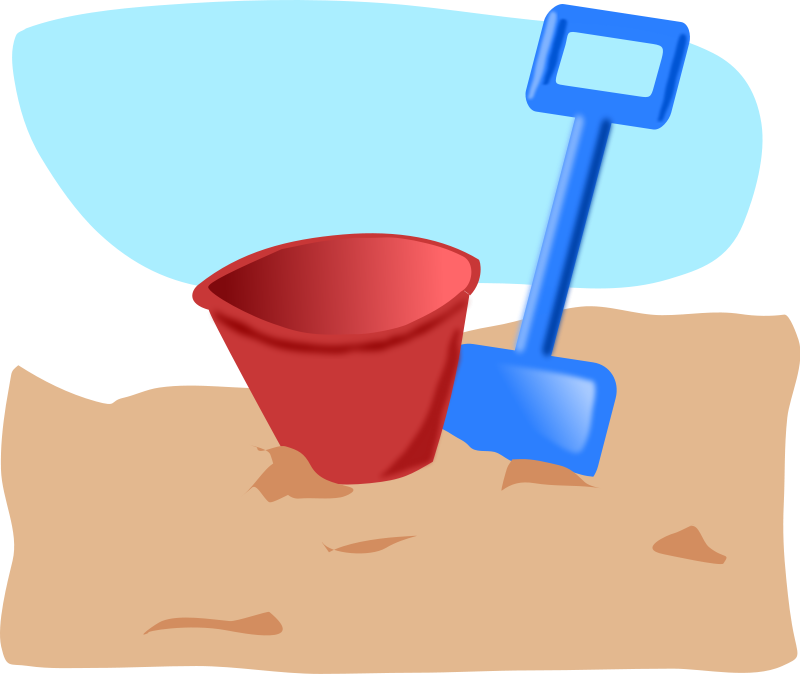
\includegraphics[width=8cm]{addon_bucket_and_spade.png}


\bigskip

\bigskip

\bigskip


\LARGE{Xinyi Chen \\ Artemi Egorov }





\bigskip

\bigskip

%\bigskip

%\bigskip

%\bigskip

Zurich\\
April 2012\\

\end{center}




\setboolean{@twoside}{true}  % change to two-side layout from here

\startnewchapter

% blank page
%\newpage
%\thispagestyle{empty}
%\mbox{}

\pagestyle{fancy}
\pagenumbering{roman}

% lesespalte 11.5 anstatt 12.5 [cm]
%\changepage{0cm}{-1cm}{0.5cm}{0.5cm}{0cm}{0cm}{0cm}{0cm}{0cm}

%---------------------------------------------------------------------------
% Preamble

%!TEX root = bericht.tex
%!TEX encoding = latin1

%---------------------------------------------------------------------------
% Abstract



\phantomsection
\addcontentsline{toc}{chapter}{Abstract}
\chapter*{Abstract}

This paper describes the principles of self-organized criticallity and their validity in cellular automation models, in particular the sandpile model. The model, its diversity, its implementation in MATLAB/Octave with different parameters and its analysis are presented in detail. RESULTS ASDF?!?


\startnewchapter

% blank page
%\newpage
%\thispagestyle{empty}
%\mbox{}

%---------------------------------------------------------------------------
% Dankssagung

\phantomsection
\addcontentsline{toc}{chapter}{Acknowledgements}
\chapter*{Acknowledgements}

The project group would like to thank the \emph{Chair of Sociology, in particular of Modeling and Simulation}, for the chance to work on an interesting project and the possibility to apply simulation skills on extraordinary topics. Special thanks go to the assistants, namely Karsten Donnay and Stefano Balietti, for their all-time support during the project. Furthermore, the group would like to thank Pegah Kassraian Fard, who unfortunately had to quit the project, for her support in the early state of the project. Additional thanks go to the other groups of the class and of previous semesters.

\startnewchapter

%---------------------------------------------------------------------------
% Symbols

%\phantomsection
%\addcontentsline{toc}{chapter}{Nomenklatur}
%\chapter*{Nomenklatur}
%\label{chp:nomenklatur}

%\section*{Abk�rzungen}
%\begin{tabbing}
%\hspace*{1.6cm}\=\kill

%STC\> standard testing conditions\\[0.5ex]
%NX\> CAD, CAE und CAM Softwarepaket von Siemens

%\end{tabbing}


\startnewchapter

%---------------------------------------------------------------------------
% Table of contents

\setcounter{tocdepth}{2}
% create a bookmark that will appear in the booksmarks displayed by
% Adobe Reader, but not in the Table of Contents of the document
\label{TOC}
\pdfbookmark[0]{Table of contents}{TOC}
\tableofcontents


\startnewchapter

%---------------------------------------------------------------------------


\pagenumbering{arabic}
\newpage

%---------------------------------------------------------------------------
% Chapters

\chapter{Introduction and Motivations}
\thispagestyle{fancy}


\ldots

\section{Cellular Automation}
A cellular automation (CA) primarily consists of
\begin{itemize}
\item a finite regular $d$-dimensional field/lattice,
\item a set of variables attached to each cell/site and
\item a set of rules that specify the time evolution of the states.
\end{itemize}
A secondary property of a CA is the fact that the evolution rules are local, i.e. the updating of a certain cell only requires information about the cell itself and its finite, bounded and well defined neighbourhood.

Further analysis of the above definitions show that a CA is deterministic, i.e. a given initial configuration will always evolve the same way. \emph{Probabilistic} cellular automata imply an external probability to drive the updating rule and therefore allow to introduce a sort of continuity, even though the automation is of discrete nature.

\section{Self-Organized Criticality}
The term self-organized criticality (SOC) basically consists of two properties:
\begin{itemize}
\item \emph{self-organization} means that a non-equilibrium system is able to develop structures on its own, without external control or manipulation.
\item \emph{criticality} implies that a local disturbance not only influences the local neighbourhood, but the whole system. In other words, all the members of a system influence each other. This term originally comes from thermodynamics and describes a state at the phase transition, where a substance (e.g. water) resides between different phases. This concept is presented in \cite{1overf}.
\end{itemize}

\section{CA and SOC}\label{sec:CAandSOC}
Generally it is difficult to determine whether a certain self-organized system exhibits self-organized criticality. One clue for a SOC-system is the existance of power-law distributions in both spacial and temporal fluctuations. Avalanche sizes (spacial) and lifetimes (temporal), as described later in section \ref{chp3:statistics}, can both show power-law behaviour of the form $f^{-a} \approx f^{-1}$.

Unfortunately, this type of correlation doesn't necesserily imply that the system is critical, i.e. non-critical systems can also show $f^{-1}$-behaviour. The key idea is that the power-law behaviour is one of the consequences of the \emph{scale-invariance} of the system. The other consequence is the presence of \emph{spacial fractals}, which is harder to identify in a dynamical system than the presence of power-law distributions.

\chapter{The Sandpile Model}
\thispagestyle{fancy}

\section{Bak-Tang-Wiesenfeld Model}

The classical sandpile model represents a cellular automation describing a dynamical system following certain rules that can be described as follows.

The field/lattice, which is chosen to be two-dimensional, represents a sandpile. Each site on the lattice has a certain value $z$ that intuitively represents the height or slope of the sandpile at certain position described with the coordinates $x$ and $y$. At each time step, a number of grains of sand is placed on top of a random site, which increases its value by a given value, e.g. one. If the value of the site exceeds a critical value $z_c$ (e.g. three), the site collapses/topples and its grains are evenly distributed to its neighbours.

In certain cases some of the adjascent sites will exceed the critical value too and the toppling process will continue until an equilibrium state is again reached. This series of collapsing sites is clasically described as an avalanche. The next grain is not placed until the equilibrium state is reached, meaning that the time scale of the random grain placement and of the development of avalanches are decoupled.

The classical model description can mathematically be represented as follows.

Initially, the lattice is empty:
\[
z(x,y) = 0 \quad\forall x, y
\]
Then, the value of a random site $x,y$ is increased:
\[
z(x,y) \to z(x_r,y_r) + 1
\]
If its value exceeds the critical value $z_c=3$, then it topples and distributes its grains to its neighbours:
\[
\begin{aligned}
z(x,y) \overset{?}{>} 3 \Rightarrow & z(x,y) \to z(x,y)-4 \\
 & z(x\pm 1,y) \to z(x\pm 1,y)+1 \\
 & z(x,y\pm 1) \to z(x,y\pm 1)+1 \\
\end{aligned}
\]

Here, we use the so-called \emph{Von-Neumann-Neighbourhood}, which consists of the four nearest neighbours. A possible alternative would be e.g. the \emph{Moore-Neighbourhood}, which consists of all eight nearest neighbours on a square lattice. One could also think of weighting the four corner neighbours to be ``further away'' from the middle cell than the four direct (Von-Neumann) neighbours.These possibilities are not discussed in this paper.

Clearly, many variations of the described model can be considered and can produce different results. The classical sandpile model, as originally described by Per Bak, Chao Tang and Kurt Wiesenfeld, represents the starting point of any further investigations considered in this paper.

\section{Parameters}
The behavior of the model is analysed dependent on different parameters such as:
\begin{itemize}
 \item lattice size
 \item number of dimensions of lattice
 \item mass conservation, i.e. if the number of grains removed from a collapsed site is equal to the sum of grains its neighbour sites received
 \item boundary conditions, see below
 \item etc.
\end{itemize}
Different types of boundary conditions can be thought of:
\begin{itemize}
 \item open: If a site near the border topples, some of its grains leave the system (mass is lost).
 \item closed: Near-border site does not fully collapse, but keeps the grains that would fall off in an open case.
 \item periodic: The system has no boundaries, i.e. toppling near the border is ``wrapped over''.
 \item mixed: E.g. the lattice is periodic in one dimension and has open boundaries in another dimension.
\end{itemize}
Figure \ref{pics:boundary} illustrates the first three basic types of boundary conditions.

\begin{figure}[!htpb]
\centering
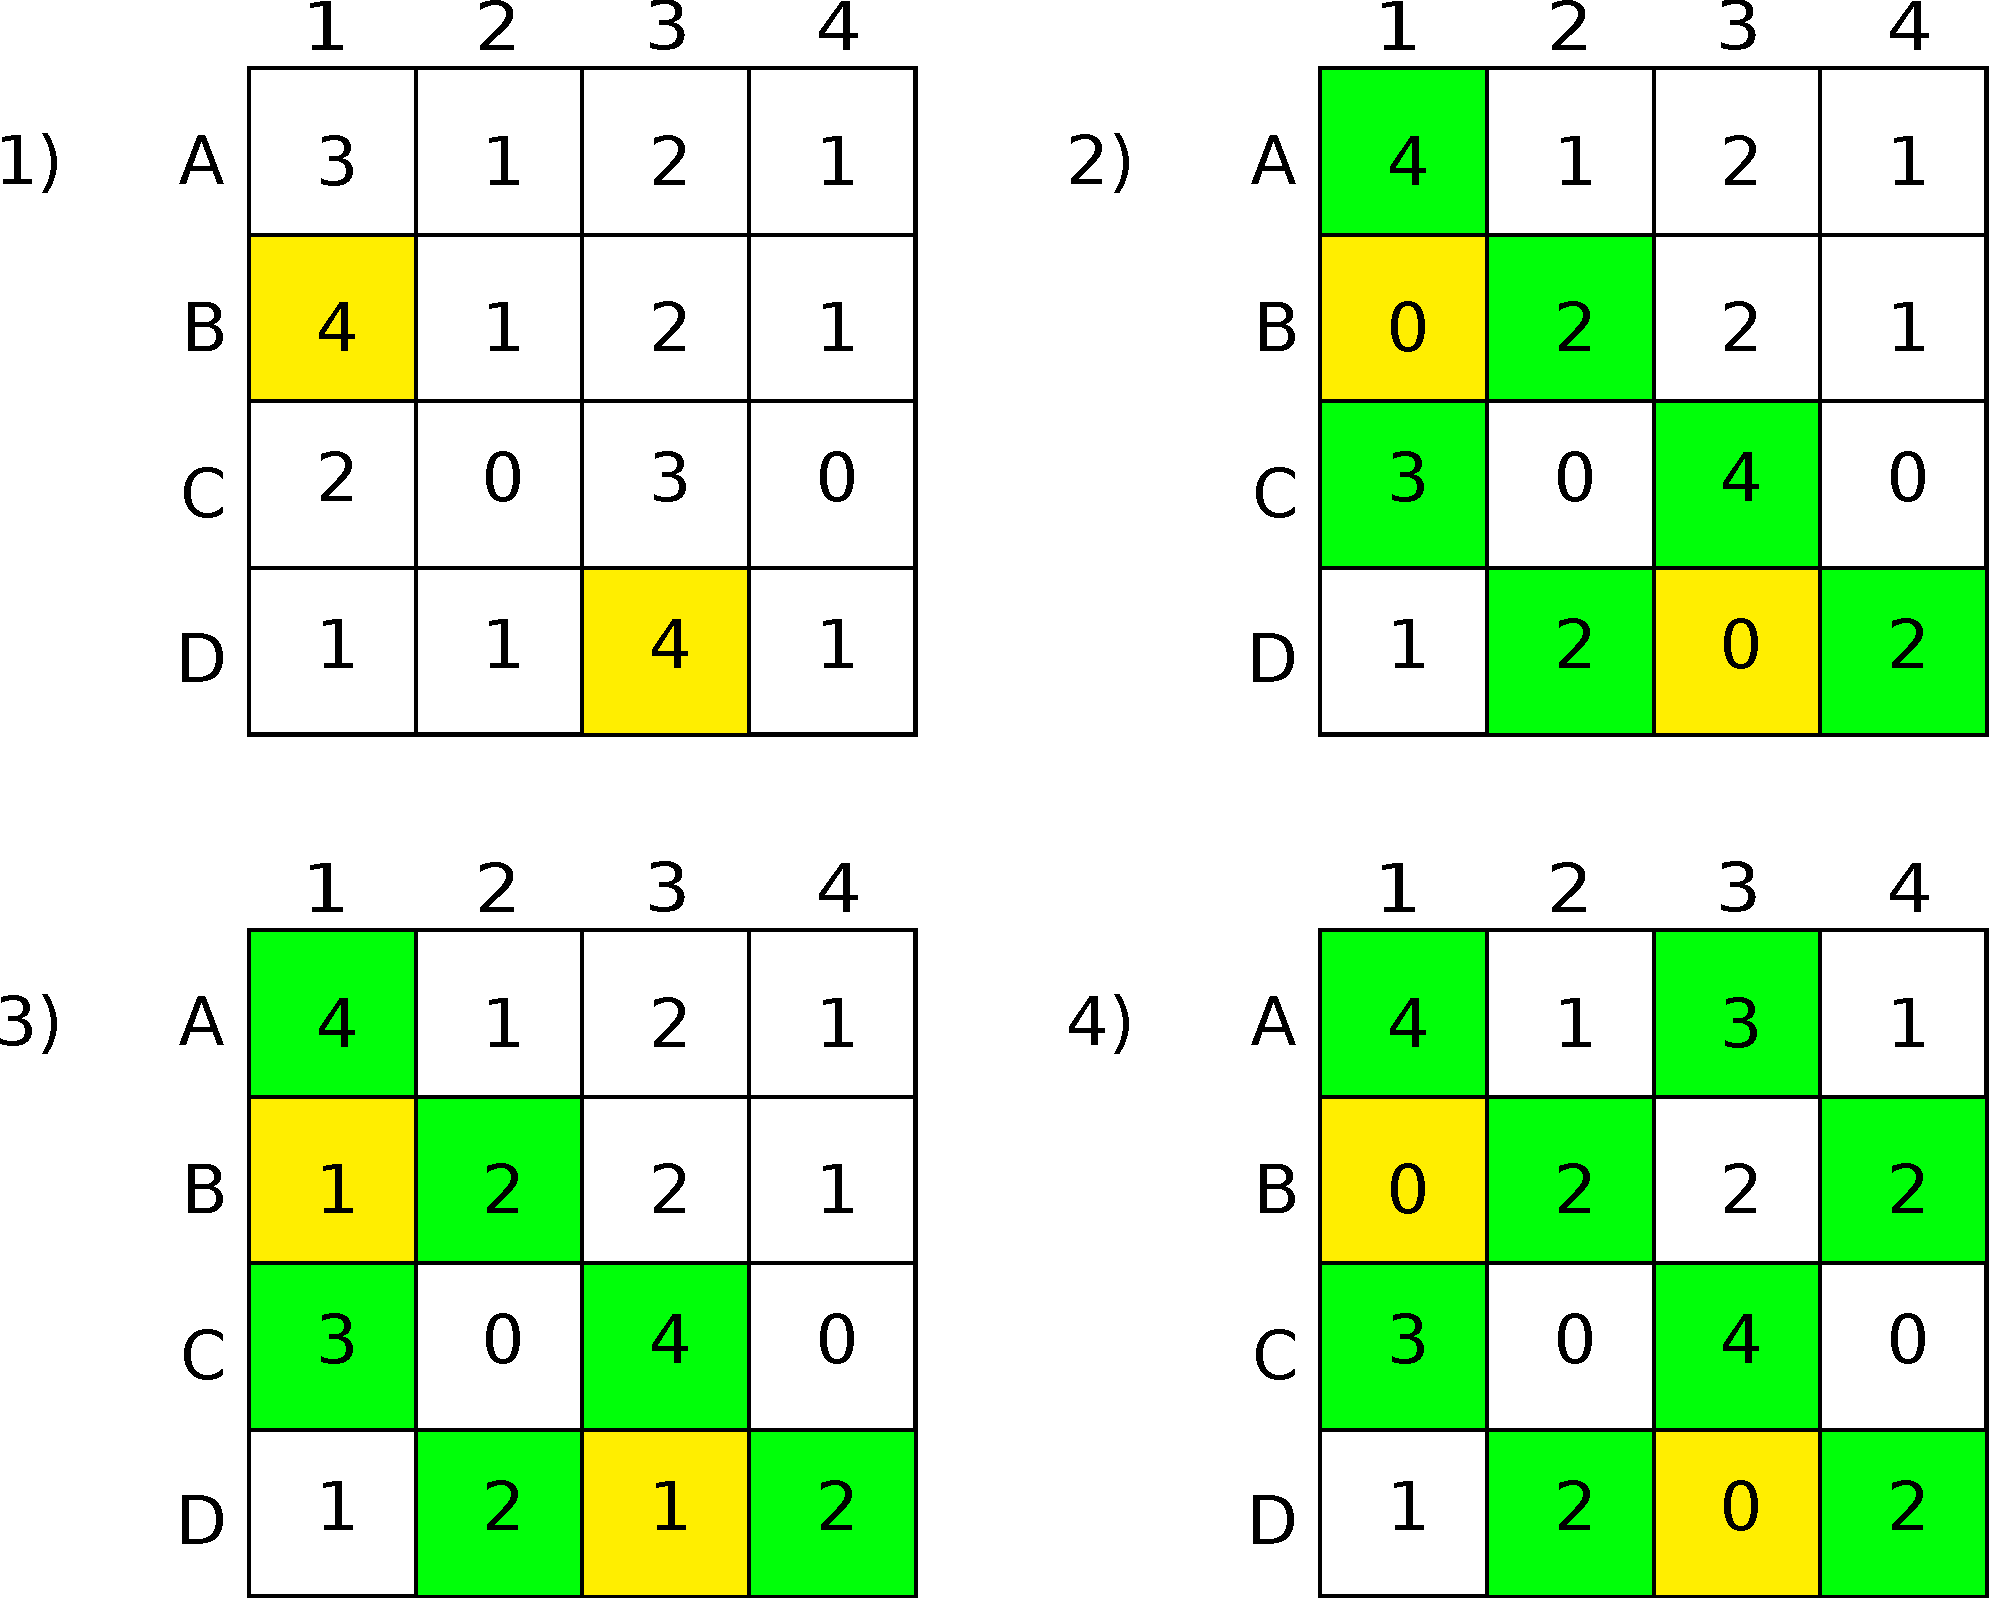
\includegraphics[width=0.5\textwidth]{pics/pic4_boundary.pdf}
\caption[]{Effect of different types of boundary conditions on a sample lattice (1): open (2), closed (3) and periodic (4)}
\label{pics:boundary}
\end{figure}

\section{Abelian Model}
One important property which can be used to categorize different sandpile models is whether they behave in a commutative or \emph{abelian} way. In particular, this can be applied to the development of avalanches in the model described above: The question posed here is, whether an equilibrium state resulting from an avalanche depends on the way the avalanche is calculated. More precisely, it can be shown that any avalanche, being a sequence of topplings, always results in the same equilibrium state i.e. does not depend on the order, in which the topplings occur. The mathematical proof of this hypothesis is nicely presented in \cite{sandpile_math}.

To illustrate this practical but not necessarily obvious fact, a sample 4x4-field with one active site is considered (see figure \ref{pics:abelian}). At step (2), two different sites simultaneously become active, therefore creating a ``choice'', which site to topple first. Depending on such choices, different sequences of topplings occur, but all lead to the same equilibrium state.

\begin{figure}[!htpb]
\centering
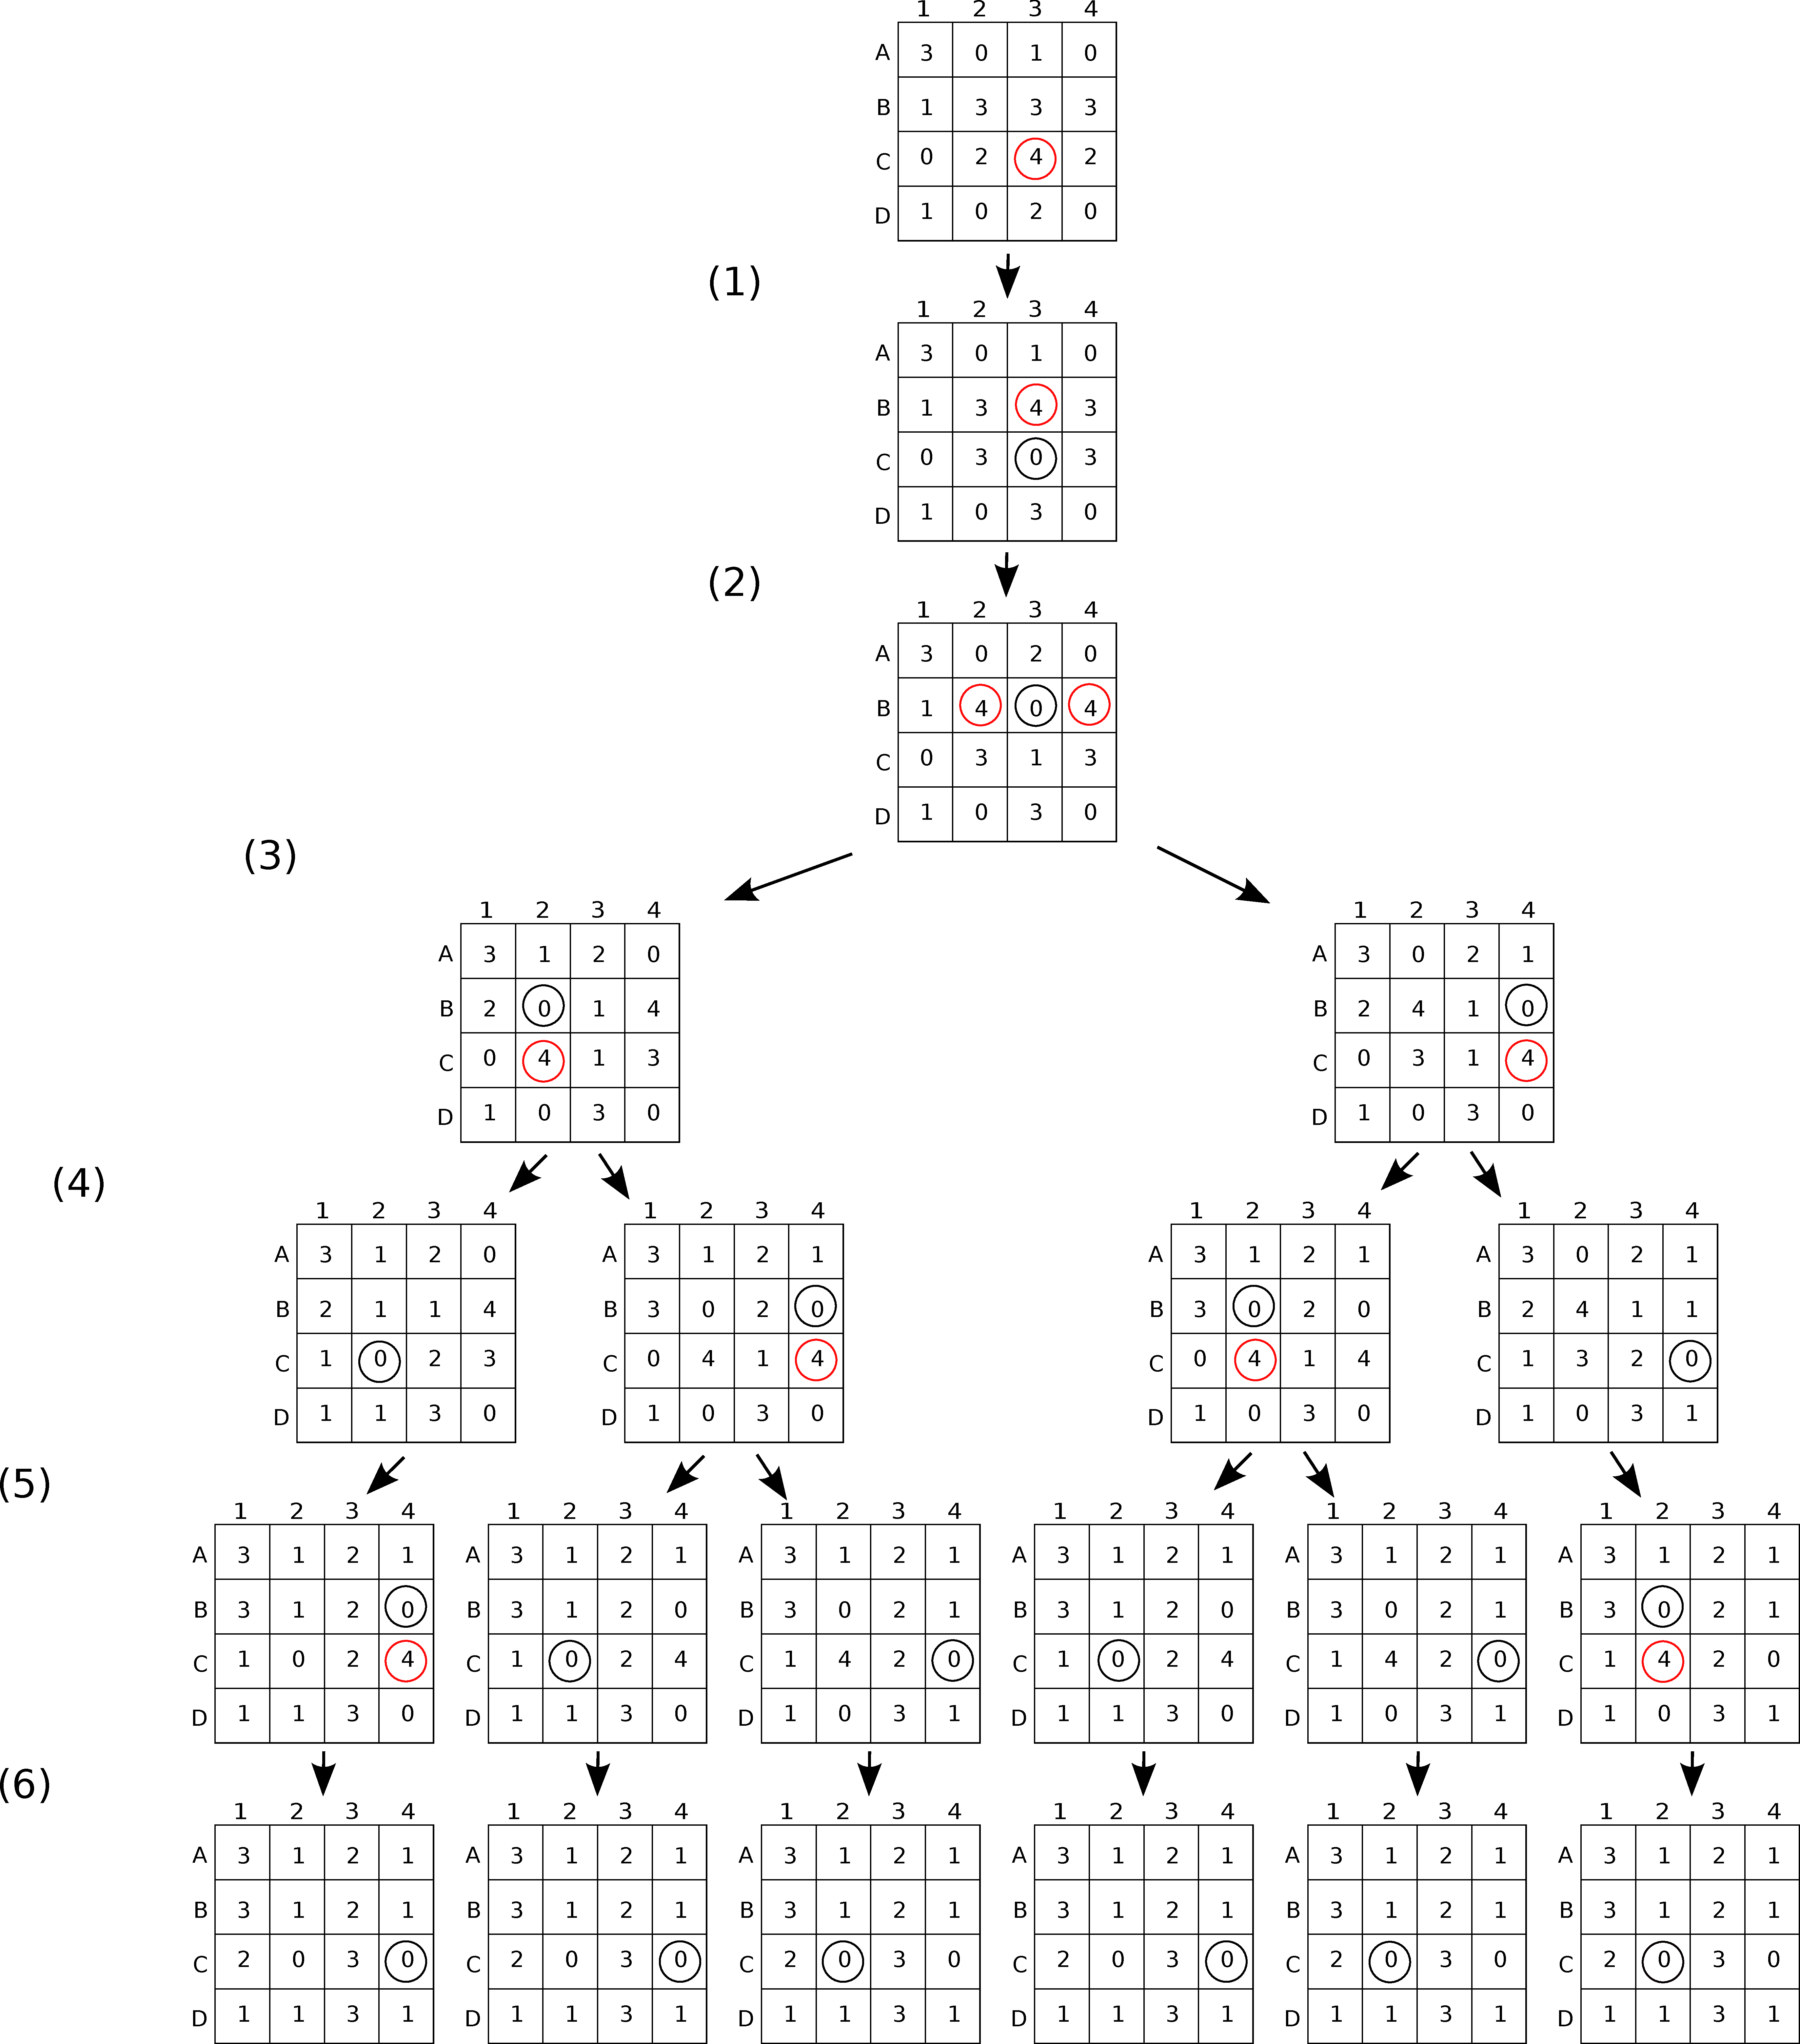
\includegraphics[width=\textwidth]{pics/pic1_abelian.pdf}
\caption[]{Demonstration of the abelian property: six different orders of topplings all lead to the same equilibrium state. The sites circled red indicate sites that have just become active, those circled black have just collapsed. Here, continuous boundary conditions have been used.}
\label{pics:abelian}
\end{figure}

\chapter{Model Implementation in MATLAB/Octave}
\thispagestyle{fancy}

\subsubsection{Note on Code and Programming Sustainability}
In order to produce  ``sustainable'' code and to share the spirit of independency coming from the open-source community, the coded routines were tested in MATLAB and in Octave (one of its open-source clones). The source code can be found in Appendix~\ref{chp:matlab}.

\section{Basic Sandpile Code}
First, a lattice/field is generated using uniformly distributed random numbers from 0 to $z_c$ (\mcode{critical_state}). This is done in order to start with a potentially critical field and not to place single grains of sand until a site gets critical.
\begin{lstlisting}
f = floor(unifrnd(0,critical_state+1,height,width));
\end{lstlisting}
Another interesting starting point is a \emph{uniform} critical field, where every site is either 0 or $z_c$.
\begin{lstlisting}
f = floor(unifrnd(0,2,height,width))*critical_state;
\end{lstlisting}

When the field is ready, a global loop runs through a defined number of timesteps, placing a grain on a random site, checking if the site becomes active and if so, computing the resulting avalanche.
\begin{lstlisting}
for t=1:timesteps
	% choose random site
	y=floor(unifrnd(1,height));
	x=floor(unifrnd(1,width));

	% place grain
	f(y,x) = f(y,x) + 1;

	% check if overcritical/active
	if (f(y,x) > critical_state)
		% avalanche code here
		% ...
	end
end
\end{lstlisting}

\section{Simple Avalanche Code}
...ASDF...

\section{Optimization of Avalanche Code}
The simple avalanche code checks the whole field including the fields, that cannot possibly be affected by the avalanche. It can therefore be optimized, for example using a LIFO data structure -- a \emph{stack}. The coordinates of very site that needs to be checked are placed on the stack, so that the computation of the avalanche consists of working through the stack and toppling all the active sites in it. During their toppling, their neighbours are again put on the stack, which makes the procedure dynamical and not easily comprehensive. The algorithm is illustrated in figure~\ref{pics:stack2}.

\begin{figure}[!htpb]
\centering
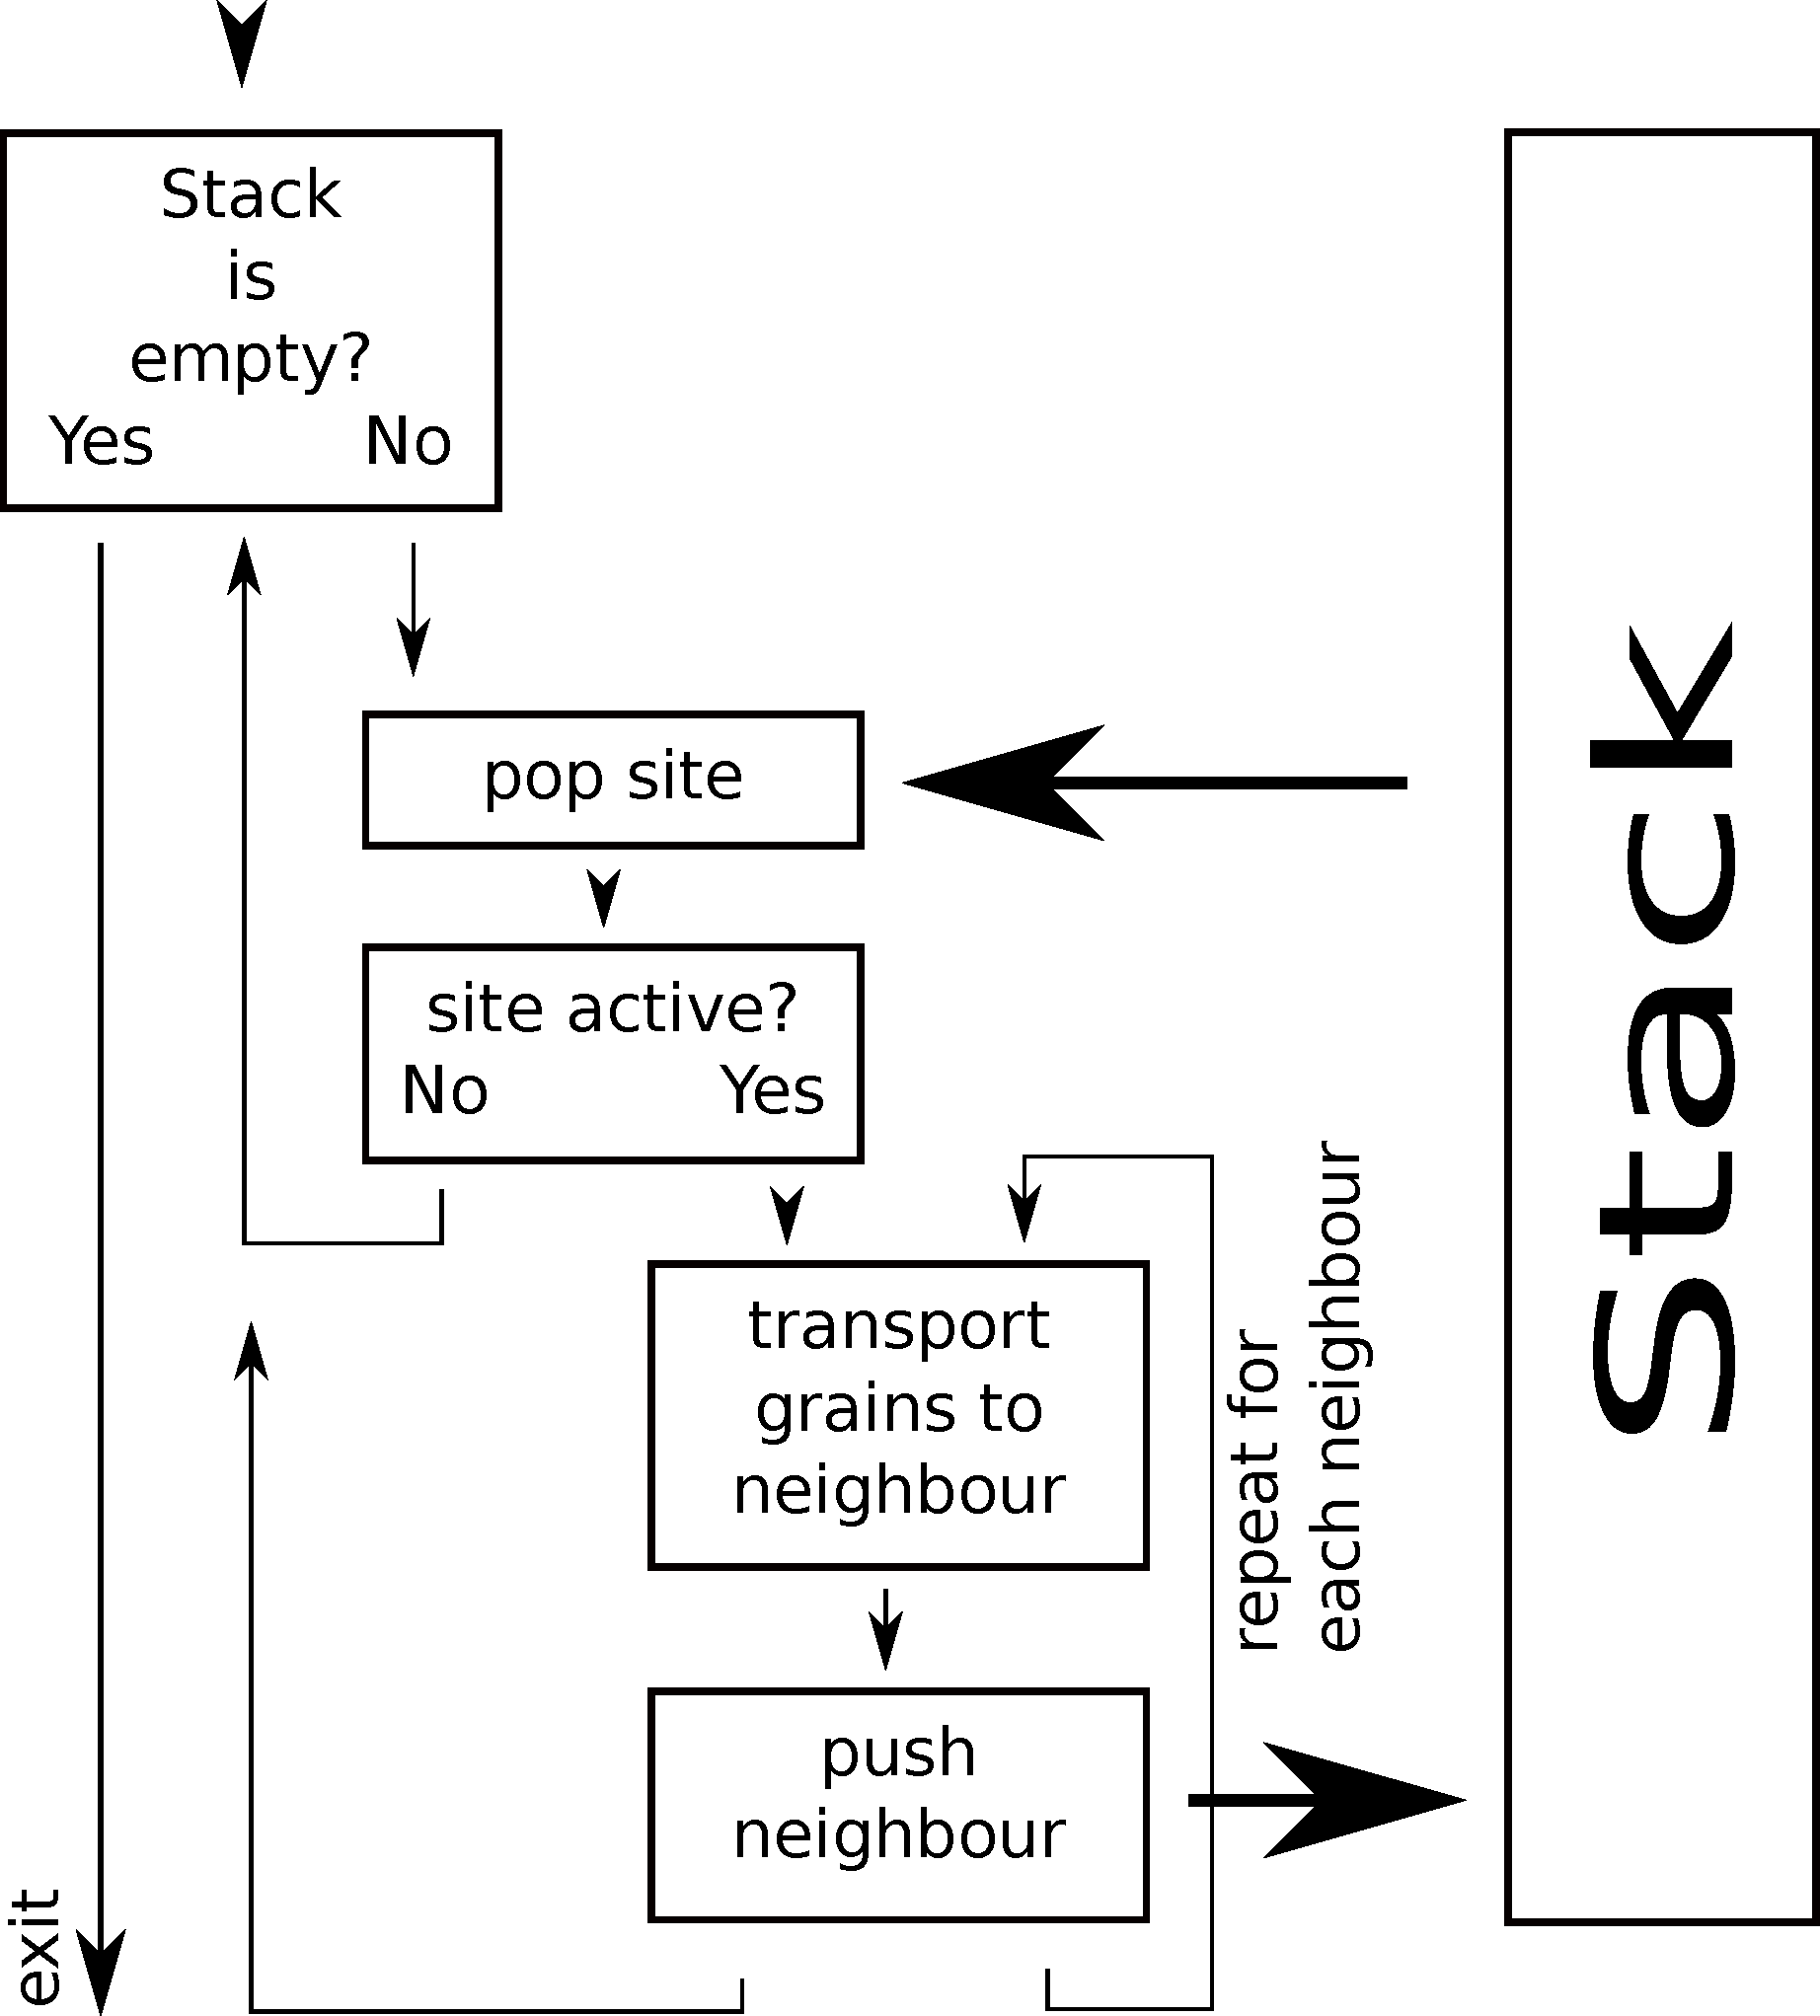
\includegraphics[width=0.5\textwidth]{pics/pic3_stack2.pdf}
\caption[]{using a stack for avalanche calculation}
\label{pics:stack2}
\end{figure}

Considering the example from figure~\ref{pics:abelian}, the stack algorithm results in the following sequence:
\begin{enumerate}
 \setcounter{enumi}{-1}
 \item push C3
 \item pop C3, topple, push its neighbours (C2,C4,B3 and D3) to stack
 \item pop B3, topple, push B2, B4, A3 and C3 to stack
 \item pop B2, \ldots
 \item pop C2, \ldots
 \item pop B4, \ldots
 \item pop C4, \ldots
\end{enumerate}
Figure~\ref{pics:stack1} shows the states of the stack after each of these steps. To avoid confusion, only the active sites are shown here.

\begin{figure}[!htpb]
\centering
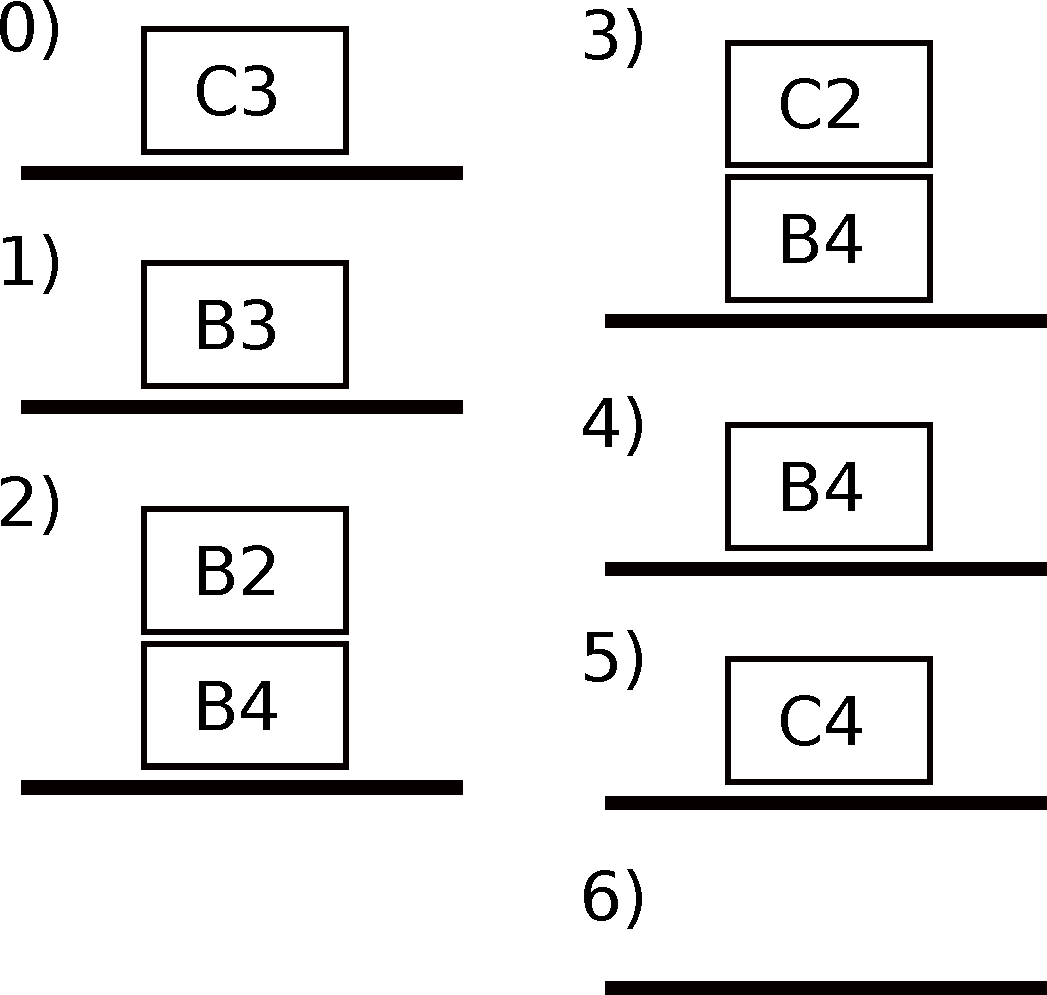
\includegraphics[width=0.5\textwidth]{pics/pic2_stack1.pdf}
\caption[]{A sample sequence of stack states. The algorithm proceeds until the stack is empty.}
\label{pics:stack1}
\end{figure}

The main loop including the stack feature looks like this:
\begin{lstlisting}
for t=1:timesteps
	% choose random site
	% ...

	% place grain
	% ...

	% push site to stack
	stack_n = 1;
	stack_x(1) = x;
	stack_y(1) = y;

	% avalanche - work through stack
	while (stack_n > 0)

		% pop from stack
		x = stack_x(stack_n);
		y = stack_y(stack_n);
		stack_n = stack_n - 1;

		% check if overcritical/active
		if (f(y,x) > critical_state)
			% collapse/topple
			f(y,x) = f(y,x) - neighbours * collapse;

			% look at every neighbour
			for n=1:neighbours
				% add/transport grain to neighbour
				f(y+neighbour_offset_y(n),x+neighbour_offset_x(n)) = ...
					f(y+neighbour_offset_y(n),x+neighbour_offset_x(n)) + collapse;

				% push neighbour to stack
				stack_n = stack_n + 1;
				stack_x(stack_n) = x + neighbour_offset_x(n);
				stack_y(stack_n) = y + neighbour_offset_y(n);
			end
		end
	end
end
\end{lstlisting}


\section{Statistics}\label{chp3:statistics}
Many different variables may be of interest for the statistical analysis of sandpile models. The easiest to implement is avalanche size:

\begin{lstlisting}
...

% check if overcritical/active
if (f(y,x) > critical_state)

	% collapse/topple
	f(y,x) = f(y,x) - neighbours * collapse;

	% record statistics
	avalanche_sizes(t) = avalanche_sizes(t) + 1;

	...
\end{lstlisting}

Here, the number of avalanches is recorded at every time step by increasing the counter after each toppling that happens during the avalanche. After the main loop, the data is sorted and the distribution is fitted into a power-law distribution given by
\[
P(s) = a \cdot s^b
\]
where $P$ is the number of avalanches of size $s$. The coefficients $a$ and $b$ are determined using a simple solver that minimizes $a \cdot s^b-P(s)$.

\begin{lstlisting}
% count avalanche sizes - calculate distribution
for s=1:max(avalanche_sizes)
	avalanche_count(s) = size(avalanche_sizes(avalanche_sizes==s),2);
end

% filter zero values
s = [1:max(avalanche_sizes)];
P = avalanche_count(1:end);
s = s(P>0);
P = P(P>0);

% fit into power-law
[c,fval,info,output]=fsolve(@(c)((c(1).*s.^c(2))-P),[100,1]);
a = c(1);
b = c(2);

\end{lstlisting}

In order to implement statistics of avalanche lifetime in the stack code, the number of additional (i.e. more than one) topplings per timestep must be counted. The reason for this is that the stack algorhithm does not follow a timescale and therefore the number of timesteps taken by an avalanche cannot be counted directly. Therefore, the following equation is used:
\[
s = \sum _t n = \underbrace{\sum_t (n - 1)}_{a} + \sum _t
\qquad \Rightarrow \sum _t = s - a
\]
where $s$ is the avalanche size, $t$ is the avalanche lifetime, $n$ is the number of topplings per timestep and $a$ is the total number of additional topplings. The neighbour-checking part of the stack loop looks like this:
\begin{lstlisting}
% count future topplings to be caused by this toppling
future_topplings = 0;

% look at every neighbour
for n=1:neighbours

	% add/transport grain to neighbour
	% ...

	% push neighbour to stack
	% ...

	% count future topplings to be caused by this toppling
	if (f(y+neighbour_offset_y(n),x+neighbour_offset_x(n)) == (critical_state+1))
		% i.e. if neighbour site becomes active
		future_topplings = future_topplings + 1;
	end

end
% calculate additional topplings caused
if (future_topplings > 0)
	avalanche_add(t) = avalanche_add(t) + future_topplings - 1;
end
\end{lstlisting}
For each toppling, the number of further topplings is counted, summed up and subtracted by one. Then, the avalanche lifetime is calculated according to the formula $\sum _t = s - a$ as follows:
\begin{lstlisting}
% return avalanche lifetimes
at = avalanche_sizes - avalanche_add;
\end{lstlisting}



\chapter{Simulation Results and Discussion}
\thispagestyle{fancy}

\section{Fractals}
As discussed in section \ref{sec:CAandSOC}, in order to show that a dynamical system exhibits SOC, some fractal nature must be present. As done analytically for a 1-D-model in \cite{fractal_avalanching}, we can plot the energy of a system over time according to the definition of normalized energy
\[
E(t) = \int_f h(x,y,t)^2 df
\]
where $h$ is the height of a site at position $(x,y)$ of the field $f$ at time $t$. In MATLAB/Octave, at the end of every main loop iteration the energy is calculated:
\begin{lstlisting}
ee(t) = sum(sum(f.^2));
\end{lstlisting}
As the energy series in 1-dimensional case shows fractal properties (see \cite{fractal_avalanching}), the question arises if this is true for a 2-dimensional case.

\section{Power-law distributions}

In this section, we investigate tha avalanche size and lifetime distribution, 
according to different boundary conditions, namely the periodic boundary conditions and open boundary conditions.



\section{Power-law distributions}

In this section, we investigate tha avalanche size and lifetime distribution, 
according to different boundary conditions, namely the periodic boundary conditions and open boundary conditions.



\subsection{Periodic boundary conditions}

For periodic boundary conditions, there is never grain lost if we do not introduce friction. 
This means that, in order to study them, we need to be careful with lattice size and driving time, 
in order to not have all the sites overcritical, which will logically imply never-ending avalanches.
As we  also need good statistics to judge the distribution, we must use a reasonably large lattice, 
though in theory, the lattice is infinite large which would imply the size should not matter.

We studied a $100\times 100$ lattice with a driving time $T=5000$, and the results are presented in the figure~\ref{sp}, 
where we see quite a nice power-law behaviour for avalanche size, but a worse one for the lifetime. 
We will give it an explanation by the end of the section, after presenting more results. 
Notice that the first point of both plot, correspond, in fact, to the case where no avalanches occur. 
It is included to show that it is more often the system stays subcritical rather than being overcritical. 



\begin{figure} 
\begin{center}
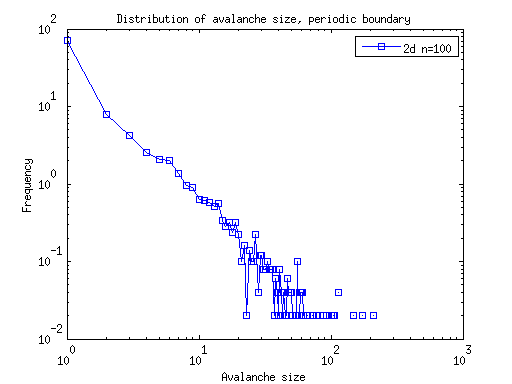
\includegraphics[width=0.49\textwidth]{results/sp.png}
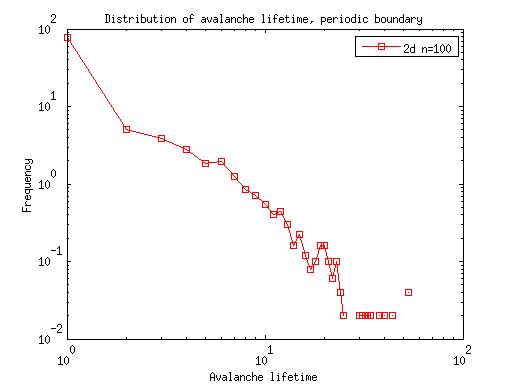
\includegraphics[width=0.49\textwidth]{results/tp.png} 
\caption{Avalanche size and lifetime distribution for $100\times100$ lattice, with periodic boundary conditions. 
The driving time is $T=5000$. }
\label{sp}
\end{center}
\end{figure} 

Due to memory-demanding large lattices and large driving time, we will not treat higher dimensions.
The periodic boundary case without grain lost, though, is not of much interest, as real systems are finite and dissipative.

Instead, we should introduce a friction parameter, and hence, consider a \emph{real} $E$ field, in contrast to a discrete integer field. 
The periodic boundary in principle implies lattice size independence, which will represent a computational advantage, as we can choose small lattice.


We studied this situation for $d=2$, with $n=10$, $n=50$ and $n=100$. See figure~\ref{spf} for the results. 
We see a clear cut-off for large avalanche number due to friction, though the we have a quite nice power-law distribution for small avalanches.
The lifetime is not shown, but it does not differ too much from the case in figure~\ref{sp}.
For the case of $n=100$, we run ten times longer than the other cases, and we see that the distribution for very large avalanches is different from small or medium-size ones. 



Figure~\ref{dsp} shows some plots for higher dimension. The cut-off effect due to friction is much less than the $2d$ lattice, 
but we can increase friction and check again its effect, see figure~\ref{3spf}.
From this analysis, clearly, the dissipation plays an important role, nevertheless, on \emph{average}, 
the total energy of lattice is kept constant when the system evolves, see figure~\ref{ep}. 

Furthermore, for $d=1$, we do not see a power-law distribution, in agreement with the prediction of theory (the situation for open boundary is also checked to be the same). Figure~\ref{1p}. 

\begin{figure} 
\begin{center}
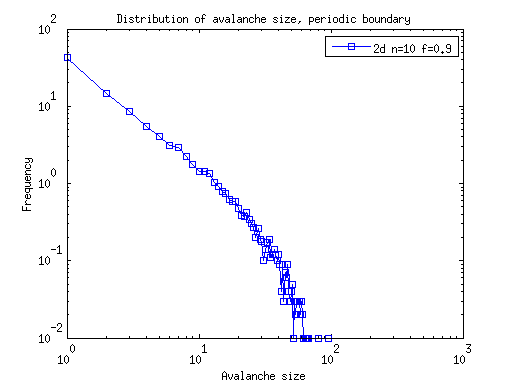
\includegraphics[width=0.49\textwidth]{results/spf.png}
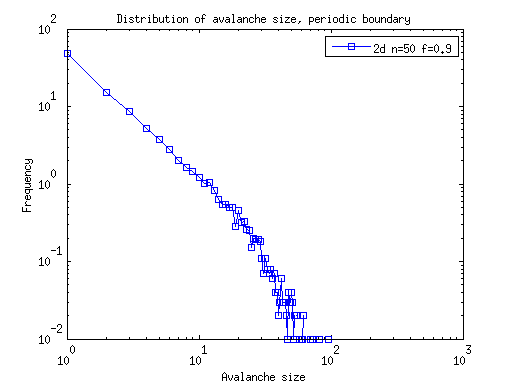
\includegraphics[width=0.49\textwidth]{results/spf50.png} \\
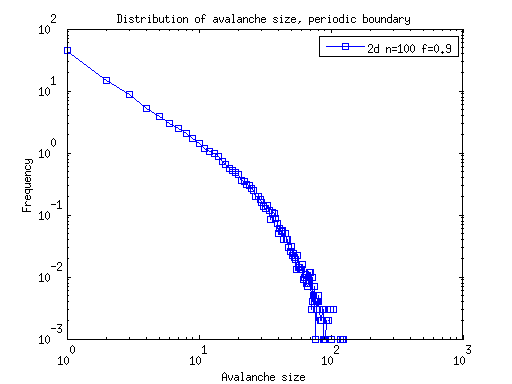
\includegraphics[width=0.49\textwidth]{results/spf100a.png}
\caption{Avalanche size distribution for $2d$ lattice with friction, with periodic boundary conditions. 
The driving time is $T=10000$ for $n=10$ and $n=50$, and $T=100000$ for $n=100$.}
\label{spf}
\end{center}
\end{figure} 



\begin{figure} 
\begin{center}
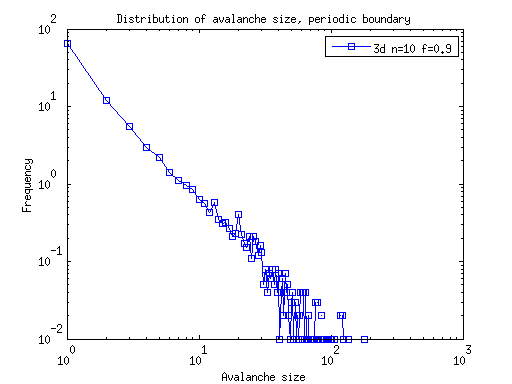
\includegraphics[width=0.49\textwidth]{results/3spf.png}
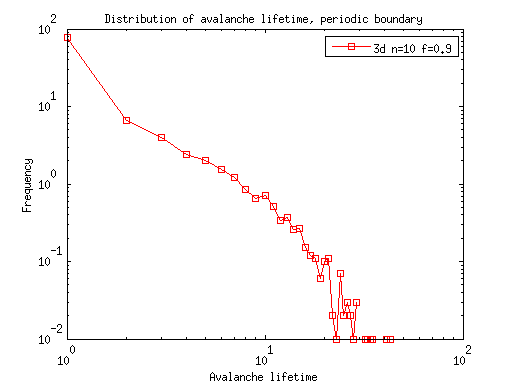
\includegraphics[width=0.49\textwidth]{results/3tpf.png} \\
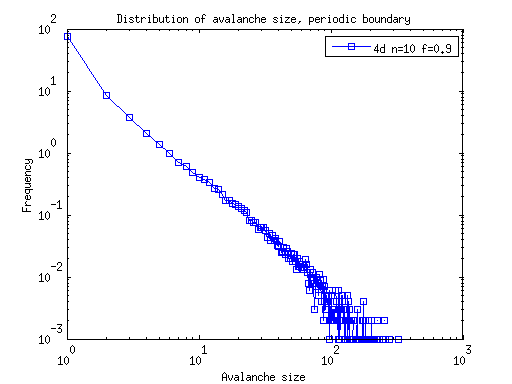
\includegraphics[width=0.49\textwidth]{results/4spf.png}
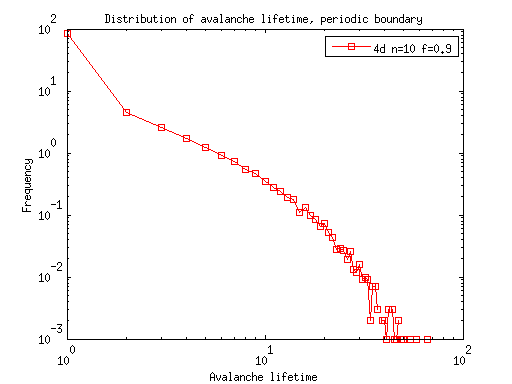
\includegraphics[width=0.49\textwidth]{results/4tpf.png} 
\caption{Avalanche size and lifetime distribution for $3d$ and $4d$ lattices with friction and periodic boundary conditions. }
\label{dspf}
\end{center}
\end{figure}  


\begin{figure} 
\begin{center}
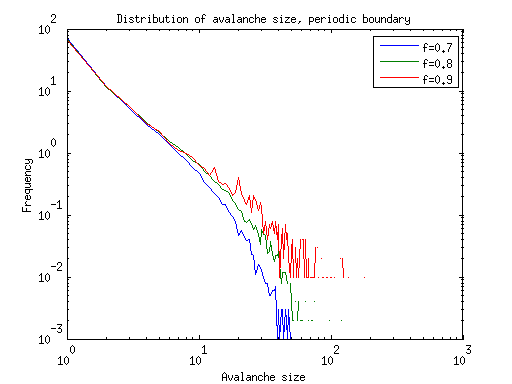
\includegraphics[width=0.49\textwidth]{results/3spfmulti.png}
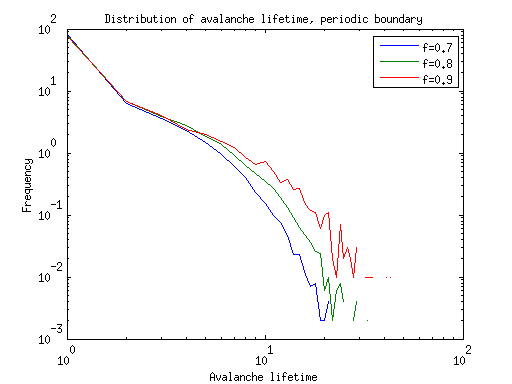
\includegraphics[width=0.49\textwidth]{results/3tpfmulti.png} 
\caption{Avalanche size and lifetime distribution for $3d$ lattice with different friction parameters and periodic boundary conditions. 
The smaller the friction parameter, the larger the dissipation. 
The first point in the lifetime distribution corresponds to zero avalanche during the lifetime.}
\label{3spf}
\end{center}
\end{figure}  

\begin{figure} 
\begin{center}
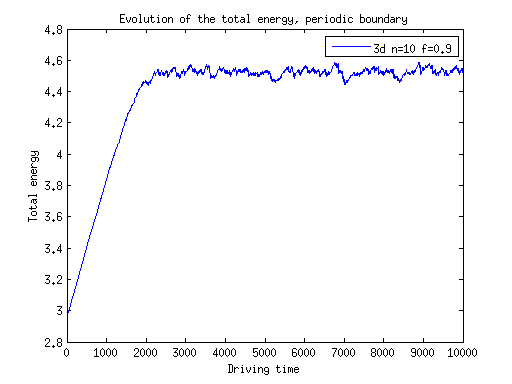
\includegraphics[width=0.49\textwidth]{results/3ep.png}
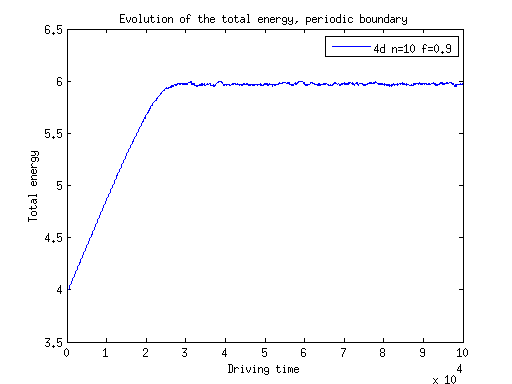
\includegraphics[width=0.49\textwidth]{results/4ep.png} 
\caption{Normalized total energy evolution for $3d$ and $4d$ lattices with friction and periodic boundary conditions. }
\label{ep}
\end{center}
\end{figure}  




\begin{figure} 
\begin{center}
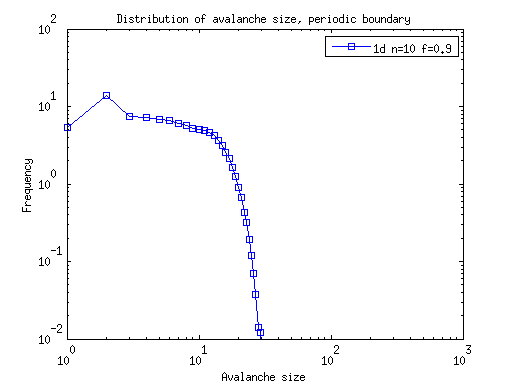
\includegraphics[width=0.49\textwidth]{results/1sp.png}
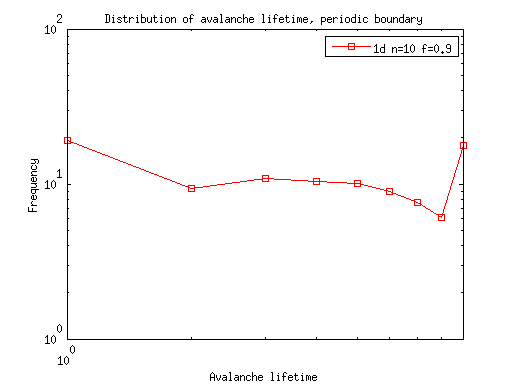
\includegraphics[width=0.49\textwidth]{results/1tp.png} 
\caption{Avalanche size and lifetime distribution for $1d$ lattices with friction and periodic boundary conditions and $T=10^5$. There is no criticality for this case. }
\label{1p}
\end{center}
\end{figure} 








A perturbation in the boundary might give a different avalanche distribution than a perturbation placed in the bulk,
as one might expect that bulk perturbation to produce bigger avalanches, 
because the grain has to be transported further in order to be lost in the boundaries.

We study this effect for 2-dimensional case, and remarkably, we do see different avalanche size distributions (figure~\ref{sv}). 
Furthermore, the high dispersion in large avalanche sizes for the bulk case causes a worse power-law distribution compared to the boundary perturbation case.

For a randomized perturbation sites, the result approaches more to the bulk one. 
\begin{figure} 
\begin{center}
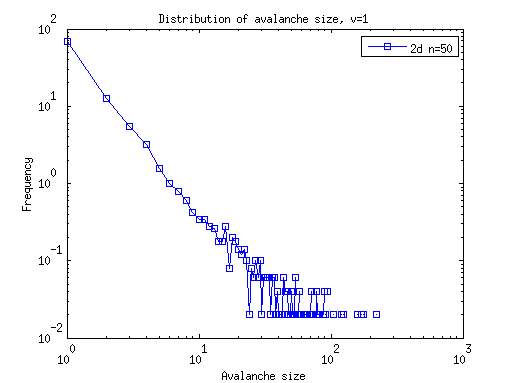
\includegraphics[width=0.49\textwidth]{results/sv1.png}
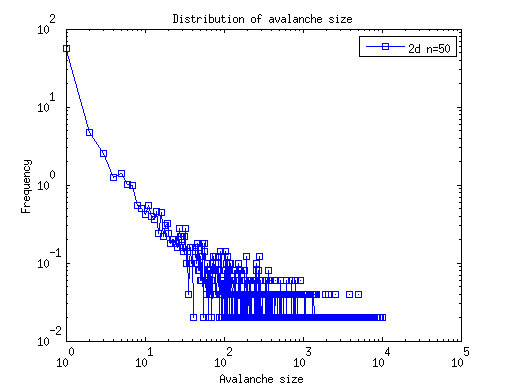
\includegraphics[width=0.49\textwidth]{results/sbulk.png} 
\caption{Avalanche size distribution for $50\times50$ lattice. 
The left one shows the result caused by perturbations in site $(1,1)$, namely in the corner; 
and right one shows the result caused by perturbations in a bulk site, $(25,25)$. The driving time is $T=5000$.  }
\label{sv}
\end{center}
\end{figure} 


The relation of the number of sites in the volume respect to the number of sites at boundary should be proportional to $n$, as it is basically the ration of volume and area.
This implies that for large lattices, one encounters much more large avalanche respect to a smaller lattice. See the plot in the figure~\ref{sn}.

\begin{figure} 
\begin{center}
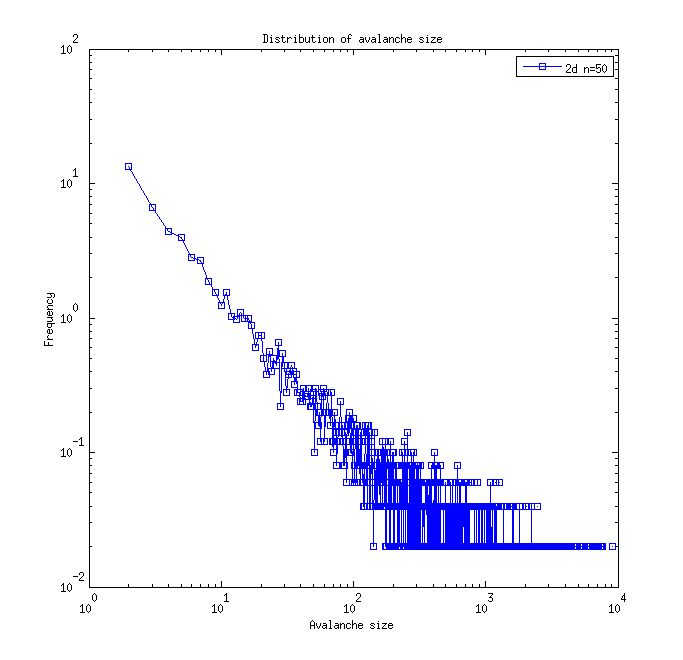
\includegraphics[width=0.49\textwidth]{results/2sn50.png}
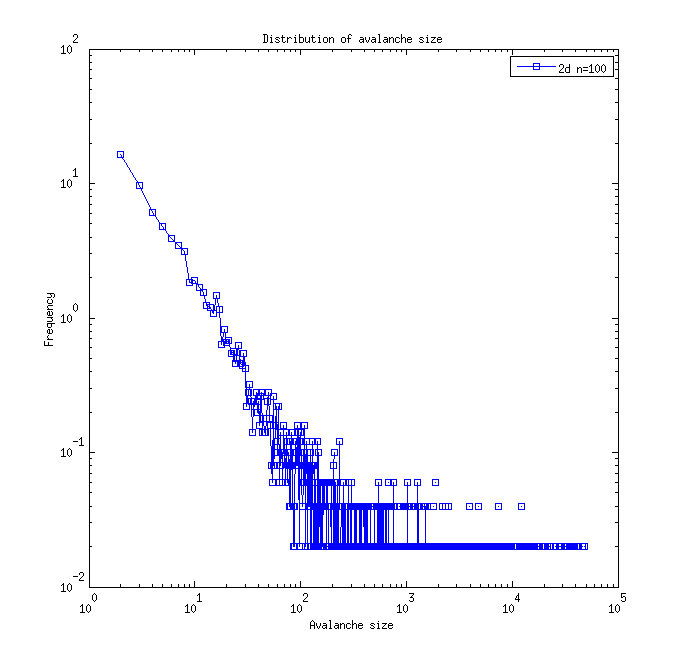
\includegraphics[width=0.49\textwidth]{results/2sn100.png} 
\caption{Avalanche size distribution for $2d$ lattices with different sizes and open boundary conditions.}
\label{sn}
\end{center}
\end{figure} 

If we add friction and go to the real case, the number of huge avalanche reduces. 
Again, we see the importance of friction to modelate the distribution to a more power-law like one, but also with cut-off effect discussed before. 
\begin{figure} 
\begin{center}
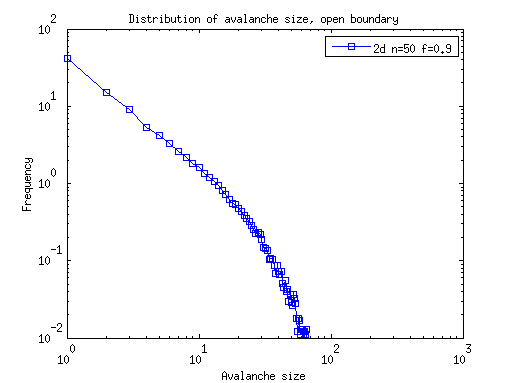
\includegraphics[width=0.49\textwidth]{results/2sof.png}
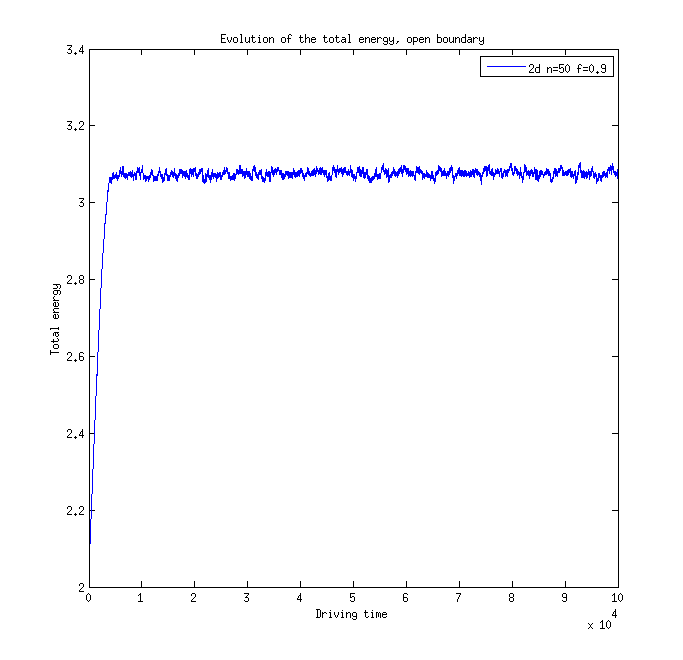
\includegraphics[width=0.49\textwidth]{results/2eof.png}
\caption{Avalanche size distribution and energy evolution for $2d$ lattices with friction and open boundary conditions.}
\label{so}
\end{center}
\end{figure} 




During the driving time, the energy of the system, namely the sum of the values of the field of all sites,
tends to oscillate around a constant value, as the additional grain in each driving time is compensated with the dissipation during avalanche, 
see for example figures~\ref{so} and \ref{ep}.





\subsection{Distribution for small lattices}

Despite we argued that many results, especially avalanche sizes distribution, showed closed to a power-law like distribution, 
except effects of friction or boundary, we here want to understand it, at least qualitatively in a more general way,
to see also why most of avalanche lifetime distribution is not power-law like.


First, let state that the total number of possible configuration states with one site ovecritical is equal to
\[
N_c=n^d\times (2d)^{n^d-1}
\]
where we think of a chain of size $n^d$ (linearize the lattice), and fix one site equal to the critical value 
(i.e. the minimal value that the site will topple, and it is set as $E_c=2d$ for convenience),
but the rest of ($n^d-1$) sites can have a value from $\{0,1, \ldots, 2d-1\}$, so $2d$ values.


However, not all of these configurations will appear during the driving time, as we randomly add only one energy grain to the system for each driving time, 
and the system can dissipate grains, this will soon lead to a characteristic average energy value per site, as we have already seen in some previous plots. 
For example, configurations such that all sites are 0 except of site is overcritical will never occur during the driving time, unless we start with it.
Thus, only a finite subset of it will occur during our simulation. 
The avalanche phenomenon (a set of configuration with one or more than one overcritical states) indeed relates this finite subset with a subset of subcritical configurations.
At contrary, the driving time (the grain adding) do the opposite relation, it makes the system be critical.
This is the mathematical struture behind it, then all the specific rules just change the number of specific site in each subsets,
like 'selecting', and this affects, obviously to the avalanches.

As we have always a discrete lattice in computation, all this relation between the discussed 2 sets exist independently if we run the system or not.
Only that, running the system, we restrict to certain subset, that for our cases, has the total energy per site close to a constant asympototic value.  
This means we just look at certain part of a full complete distribution. 

The avalanches can be characterized by its size (the total number of sites that became overcritical) 
or by its lifetime (the number of different configurations with some sites overcritical). We see that, by definition, 
the values that size can have is bigger than the values of lifetime (as the former refers to number of \emph{sites}, and the latter, to the intermediate \emph{configurations}).
One might expect that lifetime statistics converge faster to the 'exact' distribution. 

To clarify these ideas, let us consider the simplest case of discrete and small lattices with finite boundary.  
The avalanche size and lifetime distribution are shown in the figure~\ref{multi}.
We started with a initial configuration which is \textbf{minimally stable}, i.e., 
all site have a value $E_c-1$, then one grain addition in any of the site will lead to a \emph{catastrophic} avalanche, 
that affects the whole system. 
We might consider these distribution as 'exact' (the subset of 1 state overcritical configurations is almost the whole set, as the system is small enough), 
as running for even larger time, it does not change anymore. 
We can clearly see that these distributions are not power-law like, rather exponetial-like ($y=c^{-x}$). 

What happens for larger lattices is that we are restricting to small and middle large avalanches, so in some sense,
the power-law distribution is an approximation for this regime. 
Catastrophic avalanches that affect to the whole system never happens, except we impose it as initial configuration.
If we start with a zero configuration, this will neither evolve to the minimally stable state (that leads to catastrophic events). 

To check this idea, we run a bigger lattice in 2 dimension, of $50\times 50$ size, with a total driving time $T=10^6$. 
The result of avalanche size distribution is shown in figure~\ref{sfit}, with a respectable power-law fitting over two decades.
The catastrophic avalanches would have a size of order  $10^4$, which occurs for minimally stable states, which will have an average energy per site of
\[
<E>=(n^d(E_c-1)+1)/n^d=E_c-1+1/n^d
\]
which for large lattice, it is $<E>\sim E_c-1$, so $3$ for our case. We can look at the energy evolution that the system evolves to an
average energy per site around $2$ (see figure~\ref{2e}, though it starts with a random initial configuration. 
Starting with a minimally stable state will also converge to the same value).
Hence, we see that many theoretical possible states are strongly supressed. 
A small remnant which is not power-law will stay. One might first consider it as a finite size effect, 
but it is indeed a discrete effect, as we will always have this remnant for any lattice size if we run long enough time, 
due to the system is intrinsically discrete.
Nevertheless, if the system is continuous, which we cannot exactly reproduce with computer simulation, 
then, we have infinite many possible configurations and we can run infinitely large time, 
and should give a power-law distribution, no reason for it to end up abruptly.
Of course, this is our intuition, and it should be proven mathematically, which we will not do this in this project.
Our discussion is only in the qualitative level, that should help to understand better why cellula automata model of sandpile 
generate power-law like distribution.

We saw in some previous plots an accumulated large amount of large events, but also with a lot of dispersion, 
this is mainly statistical fluctuations. 
Running large enough time, this effect shoul go away and have a distribution like in figure~\ref{sfit}, compare it with the plots in figure~\ref{sn}, where $T$ mush smaller.

Let us now discuss a bit more about the lifetime distribution.  We saw that, quite robustly, it keeps its shape for all the different cases we studied.
The catastrophic avalanches do not have the largest lifetime, and normally, the largest value of lifetime is much less than the total site, unlike avalanche size that can outnumber it.
We show in a table~\ref{tabn2} of catastrophic avalanches in 2 dimensional lattice, and see that the maximum avalanche size is of the order $n^d$, where the lifetime is of the order $n\cdotd$.
Therefore, lifetime should converge faster than avalanche size.

Finally, some last comments on the random set up during the driving time. 
If we always place one grain in the same position in each driving time, 
this will certainly lead to limit cycle, where a finite set of configurations will keep repeating themselves. These states are called recurrent states.
The existence of limit cycles is proven analytically using the abelian property (see Dhar), and we also check it for small lattices, for example
\[ \left( \begin{array}{ccc}
3 & 2 & 2 \\
3 & 4 & 3 \\
0 & 1 & 3 \end{array} \right)\] 
Adding always a grain to the center, a finite configurations repeats. The reader can check it easily by hand or using the \texttt{abelian_sandpile.m} program, 
that can also show the intermediate configurations. This in fact happens to any initial configuration that are attracted to the corresponding limit cycle (they are many different limit cycle depending on where you place the grain).
Furthermore, for periodic boundary condition, with only one grain, the system will infinitely goes into loop between these configurations (maybe this picture corresponds better to the limit cycle notion).
Using randomized grain adding avoids this kind of situation, which are due to discreteness. 





\begin{figure} 
\begin{center}
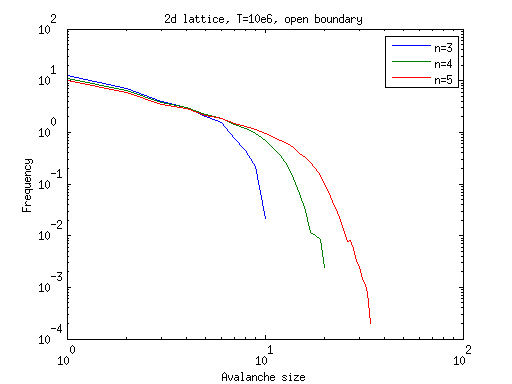
\includegraphics[width=0.49\textwidth]{results/smulti.png}
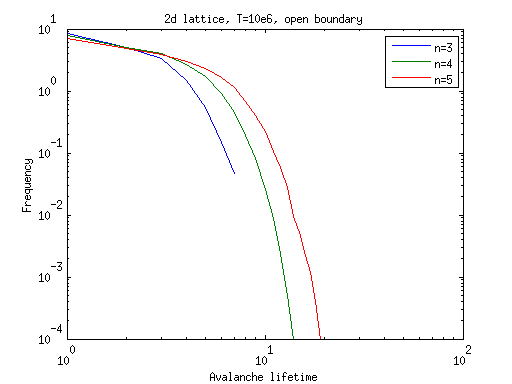
\includegraphics[width=0.49\textwidth]{results/tmulti.png}
\caption{Avalanche size and lifetime distribution for $2d$ small lattices, 
which it started with the all the sites critical. 
These distributions are checked to fit quite well with exponential decaying distributions,
the fitting parameters are not shown, as their value are not meaningful for our discussion.}
\label{multi}
\end{center}
\end{figure} 


\begin{figure} 
\begin{center}
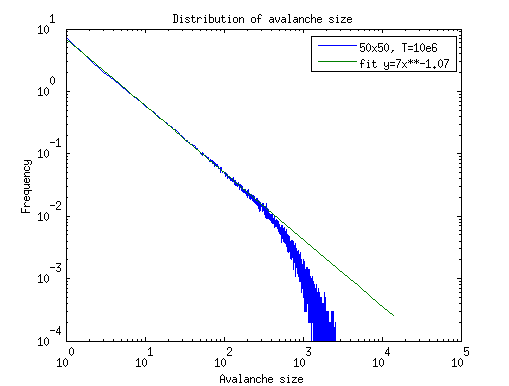
\includegraphics[width=0.49\textwidth]{results/2dsfit.png}
\caption{Avalanche size distribution for $2d$ lattice. }
\label{sfit}
\end{center}
\end{figure} 

\begin{figure} 
\begin{center}
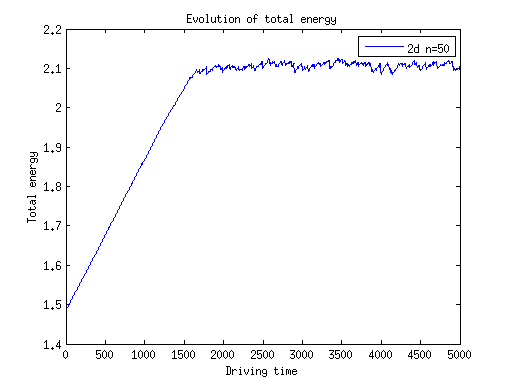
\includegraphics[width=0.49\textwidth]{results/2e.png}
\caption{The evolution of the total energy per site for $2d$ lattice, starting with a random configuration. }
\label{2e}
\end{center}
\end{figure} 

\begin{center}
\begin{tabular}{|c|c|c|c|}
 \hline
 n                  & site  & av. size & av. lifetime\\\hline
 \multirow{3}{*}{3} & (1,1) & 9        & 5 \\ \hline
                    & (1,2) & 9        & 4 \\ \hline
                    & (2,2) & 10       & 3 \\ \hline
 \multirow{3}{*}{4} & (1,1) & 16       & 7 \\ \hline
                    & (1,2) & 16       & 6 \\ \hline
                    & (2,2) & 21       & 5 \\ \hline
 \multirow{6}{*}{5} & (1,1) & 25       & 9 \\ \hline
                    & (1,2) & 25       & 8 \\ \hline
                    & (1,3) & 25       & 7 \\ \hline
                    & (2,2) & 34       & 7 \\ \hline 
                    & (2,3) & 34       & 6 \\ \hline
                    & (3,3) & 35       & 5 \\ \hline
\end{tabular}
\caption{Table with catastrophic avalanches, where the \emph{site} refers to the critical site, while other sites are minimally stable (with value $E_c-1$).}
\label{tabn2}
\end{center} 
\chapter{Summary and Outlook}
\thispagestyle{fancy}

Self-Organized Crititicaly (SOC) was born as a new mechanism to produce power-law behaviour, as this latter is common in many complex systems. 
We motivated us to understand the underlying idea behind the concept of SOC and we focused on the Abelian Sandpile Model (ASM),
as this is the simplest model and also, the most popular in the literature. 

We wrote our own program of ASM to investigate its properties, particulary, simulating the avalanche behaviour for different parameters of the model, e.g.
the boundary conditions or the dimension of the cellula automaton lattice. We measure the observables of the avalanche size and avalanche lifetime, 
which are claimed to obey power-law-like statistics in literature. 

The results were, most of the time, close to power-law, especially for the avalanche size distribution. 
Nevertheless, this does not really give a better insight to the meaning of either self-organization nor criticality. 
In fact, despite a large amount of publication in this field, SOC is still a vague concept with many controversies. 
For example, many authors relate the power-law behaviour to fractal structure which is not proven, and seemingly, wrong. 

From this study, we formed our own interpretation of SOC. 
Let us start discussing the cellula automaton of ASM, which is always a discrete system, even though we made the field 'real' 
(the number of decimal is finite, so multiply it to the corresponding decimal power, we get the discrete lattice, then, instead of thinking in terms of adding or toppling one grain, 
we do for lots of grains, but relatively small respect to the total amount in the system).
As it is discrete and finite, there is a finite number of all the possible configurations.
The 'critical' behaviour is implemented by construction to the model, meaning that there exists a critical value to the field that we associate to each lattice point, where beyond it,
we let the site relax obeying certain \emph{local} rules, in our case, distributing some value of 'toppling' field to its nearest neighbours, which themselves might also be overcritical and relax.
This is the so-called avalanche effect. 

In general, we can say that the avalanche effect is due to the existence of a critical value and a local propagation rule.
With \emph{local}, we refer that the overcritical site relaxs, but not necessary to the nearest neighbours, but also possible to any random sites.

The many different cases that we treated, either open or close or periodic boundary condition with friction or not, all can be understood conceptually in the same way.

We conclude that avalanches connect the set of configurations with one overcritical site to the set of subcritical configurations.
As we have a finite total configurations, in principle, an exact distribution of avalanche size or lifetime exists. 
The driving time, by adding grains (randomly or not) brings a subcritical state to an overcritical state,
hence, if we run long enough time, we may pass through all finite configurations, and therefore, plot the distribution in an accurate way.

We did for a small lattice with a driving time comparable with the total possible number of critical configuration, 
in 2, 3 and 4 dimension, and the result is striking, as it is not a power-law, rather than a kind of exponential law. 

How can we, though, relate to the power-law results obtained for the many cases that we dealt with? 
The answer is quite simple. In all these cases, we studied whether large lattices or introduced friction or make the field real. 
Indeed, all this small changes to the model are equivalent to a discrete lattice with some different local rules, but they share a common thing,
which is to increase the number of critical configurations and also subcritical or metastable configurations.
As the random energy addition and dissipation evolves and oscillates to some constant average value,
we bearly cannot reproduce the total 'exact' distribution, unless using a total driving time comparable with all possible configurations of the system, which is a combinatorial number. 
Hence, for large lattices it is impossible computationally and we usually get the small or medium size avalanches. 
The power-law distribution is really a good approximation for this part. 
The different cases just specify a particular way to connect the set of critical configurations to the subcritical set. 

It should also be possible to treat it analytically exploiting the symmetry of the lattice, and deduce a general large lattice law, 
tending probably to a power-law approximation, as this will correspond to reducing the 'finite size' effect or to the 'continuous' limit. 
We do not know if this is done, but certainly, it will be a nice result and save also some computational power. 


Where is the criticality, then? First, let us recall the meaning of criticality. This is a concept borrowed from thermodynamic systems 
that undergo a 2nd order phase transition (e.g. spontaneous magnetization below Curie temperature), 
which imply the correlation length to diverge, i.e., all the system, independent of size, behave together in the same way, 
hence, we can say there is no a characteristic scale during the phase transition.


For our ASM, we really do not have this kind of phenomenon.  
What we have is a metastable configuration that goes critical by an external input and then relaxes to another metastable configuration,
but there is a large number of different metastable configurations. The avalanches connect to each other and their statistical distribution of power-law-like behaviour, 
as we discussed, so we dare to conclude there is no criticality in the sense of thermodynamic systems. 

Regarding the self-organization, the system does not self-organize itself to a particulary interesting state, like the case of magnetization, where all the spins point to one direction.
In fact, if one always input the energy or grain in the same site, it can be proven that there exists a limit cycle, i.e. there is a finite number of configurations that repeat again and again, infinitely.
Hence, we might also refute the self-organization, as the system needs external input to organize to some critical state, their relaxation just gives one of many metastable subcritical state.

The term SOC is, hence, might not seem very appropiate. Nevertheless, this model is useful to understand many real systems in nonequilibrium.
Systems in nonequilibrium are open systems, thus they receive external input, and because of this, they might undergo to different metastable states, especially
for large but slowly driven systems with possibilities of dissipation (avalanche). 
Think for example the earthquake model, where the earthquake is the avalanche of the system, that releases energy when it finishes and bring the system back to a metastable state, 
then the system will be slowly driven again to a critical state, and so on and so forth. The statistics of earthquakes size will follow power-law distribution. 
Note as well that this system would be considered continuous.

In conclusion, slowly driven systems with avalanche phenomenon can be modelled by computational sandpile models, and we can refer this kind of real systems as SOC systems.
However, the name of SOC is not really appropiate, as the system is slowly driven to a critical state that relaxes itself with the avalanche phenomenon, and the process is repeated again.
The statistics of avalanche for such a continuous system seems to be power-law like, as it is checked by computer simulations. 





%\include{}
%\startnewchapter




%---------------------------------------------------------------------------
% Literature
% (create .bib files using, for example, the free application Jabref)
% Compile your report in the following order: latex - bibtex - latex - latex
%\startnewchapter
\bibliographystyle{plain} % jurabib
\phantomsection
\addcontentsline{toc}{chapter}{References}
\begin{flushleft}
\bibliography{bibliography}
\end{flushleft}
\thispagestyle{fancy}

%---------------------------------------------------------------------------
% Appendix
\startnewchapter
\appendix
%!TEX root = bericht.tex
%!TEX encoding = latin1




%---------------------------------------------------------------------------

\startnewchapter

\chapter{MATLAB/Octave-Code}\label{chp:matlab}
\thispagestyle{fancy}
% NOTE: to change font size refer to mcode.sty

\section{``critical field.m'' - random field generation}
\lstinputlisting[frame=tb]{../../code/critical_field.m}
\vspace{2em}

\section{``sandpile.m'' - 2D sandpile model simulation, parametrized}
\lstinputlisting[frame=tb]{../../code/sandpile.m}
\vspace{2em}

\section{``avalanche distribution analysis.m''}
\lstinputlisting[frame=tb]{../../code/avalanche_distribution_analysis.m}
\vspace{2em}

\section{``test sandpile.m'' - sandpile simulation test environment}
\lstinputlisting[frame=tb]{../../code/test_sandpile.m}
\vspace{2em}

\section{``abelian sandpile.m'' - n-dimensional sandpile simulation w. friction}
\lstinputlisting[frame=tb]{../../code/xinyi/abelian_sandpile_XY.m}
\vspace{2em}

\section{``coordinate.m''}
\lstinputlisting[frame=tb]{../../code/xinyi/coordinate.m}
\vspace{2em}

\section{``linear index.m''}
\lstinputlisting[frame=tb]{../../code/xinyi/linear_index.m}
\vspace{2em}

\section{``neighbour.m''}
\lstinputlisting[frame=tb]{../../code/xinyi/neighbour.m}
\clearpage

%\section{Photothermie.m\cite{tyfocor}}
%\lstinputlisting[frame=tb]{matlab/photothermie1.m}
%\clearpage

%\section{Diffgleichung.m}
%\lstinputlisting[frame=tb]{matlab/photothermie2.m}
%\vspace{2em}



%---------------------------------------------------------------------------

\startnewchapter

%\chapter{Daten Oerlikon Solar PV-Modul}\label{appendix:oerlikon}
%\thispagestyle{fancy}

%\begin{itemize}
%\item Dimensionen: $1.1 \times 1.3$~m
%\item Wirkungsgrad: 8~\% (bei STC)
%\item Temperaturkoeffizient: -0.29~\%/K
%\end{itemize}

%\includepdf[pages=-]{pdfs/globalsolar_G2_Thin_Film_String_Datasheet.pdf}

 


\end{document}
%===========================================================================
